%# -*- coding: utf-8-unix -*-
%%==================================================
\chapter{自然语言理解}\label{SSPChapter8}
%%%%%%%%%%%%%%%%%%%%%%%%%%%%%%%%%%%%
\begin{tcolorbox}[colback=white!50,colframe=orange!50,title=自然语言]
\begin{center}
自然语言是指人类日常交流所使用的语言。自然语言理解主要研究如何使计算机能够理解和生成自然语言。自然语言理解既是人工智能研究较早的一个领域, 同时也是现代计算机的一个必备特征. \hfill
\end{center}
\end{tcolorbox}
%%%%%%%%%%%%%%%%%%%%%%%%%%%%%%%%%%%%
%%%%%%%%%%%%%%%%%%%%%%%%%%%%%%%%%%%%%%%%%%
\begin{figure}[H]
\centering

\includegraphics[width=0.86\textwidth]{NLP20191218008.jpg}
\caption{}
\label{NLP20191218008}
\end{figure}
%%%%%%%%%%%%%%%%%%%%%%%%%%%%%%%%%%%%
2020年1月, NLP的抱抱脸(hugging face)团队发布了新资源!帮助NLP过程中词语切分(tokenization)更快的库\href{https://github.com/huggingface/tokenizers}{Tokenizers}.
只要20秒就能编码1GB文本,适用Rust、Python和Node.js,已经在GitHub上获得了800多星.

在NLP模型训练中,词语标记和切分往往是一个瓶颈. Tokenizer能够训练新的词汇,并且进行标记.
功能多样:适用于BPE/byte-level-BPE/WordPiece/SentencePiece各种NLP处理模型
可以完成所有的预处理:截断(Truncate)、填补(Pad)、添加模型需要的特殊标记.
速度超级快:只需要20秒就可以在CPU上标记1GB的文本.
目前适用三种编程语言:Rust/Python/Node.js.

github的资源页面上提供了在Python上使用Tokenizers的示例,进行简单的设置就可以使用, 目前可用于三种语言Python、JS、Rust.
%%%%%%%%%%%%%%%%%%%%%%%%%%%%%%%%%%%%%%%%%%%%%%
\paragraph{Transformer 架构}
广泛用于自然语言处理中,并且在许多任务中实现了 sota(「state-of-the-art」, 用于描述机器学习中取得某个任务上当前最优效果的模型). 为了获得这些结果,研究者不得不开始训练更大的 Transformer 模型。在最大的配置中,参数数量已经超过了 0.5B/层,层数多达 64。

诸如此类的大型 Transformer 模型频频出现,到底是客观上必须要求如此多的资源,还是仅仅是因为处理效率不够高?

如果说每层的内存占用只有这么一些的话,部署 Transformer 会比实际中更容易,但是事情并不是这样的。以上的估计只包括了每层的内存占用情况和输入的激活损失,并没有考虑 Transformer 上的内存占用问题:


由于激活需要被存储并用于反向传播,有着 N 层的模型的大小比单层大了 N 倍;

由于中间的全连接层的深度 d\_ff 通常远大于注意力激活层的深度 d\_model,因此需要占用很大的内存;

在长度为 L 的序列上的 attention 的计算和时间复杂度是$O(L^2)$,所以即使是一个有 64K 字符的序列就会耗尽 GPU的内存。

研究者提出了一种 Reformer 模型来解决刚才说的那些问题:

可逆层(Reversible layer),在整个模型中启用单个副本,所以 N factor 就消失了;

在前馈层(feed-forward layer)分开激活和分块处理,消除 d\_ff factor,节省前馈层的内存;

基于局部敏感哈希(locality-sensitive hashing,LSH)的近似注意力计算,让注意力层的$ O(L^2)$因子替代$ O(L)$因子,实现在长序列上的操作。

$\bullet$\href{https://openreview.net/pdf?id=rkgNKkHtvB}{Pytorch implementation of Reformer}. It has been validated with a toy auto-regressive task.

Install (如图\ref{PycharmPytorchReformer})

>>>pip install reformer\_pytorch
%%%%%%%%%%%%%%%%%%%%%%%%%%%%%%%%%%%%
\begin{figure}[htbp]
\centering
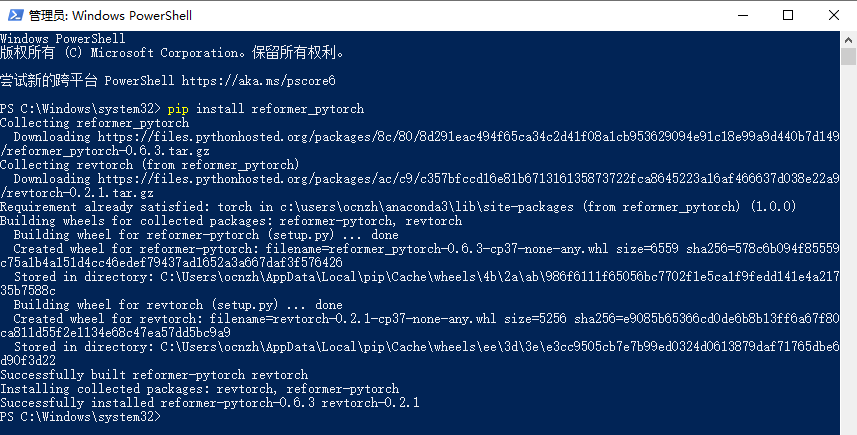
\includegraphics[width=0.9\textwidth]{Reformerpytorch0118.PNG}
\caption{Reformer安装}
\label{PycharmPytorchReformer}
\end{figure}
%%%%%%%%%%%%%%%%%%%%%%%%%%%%%%%%%%%%%%%%%%%%%%
\section{语言及其理解的基本概念}
自然语言是音义结合的词汇和语法体系. 词汇是语言的基本单位, 它在语法的支配下可构成有意义和可理解的句子, 句子再按一定的形式构成篇章等. 其结构如图\ref{AI32fig3001}所示:
%%%%%%%%%%%%%%%%%%%%%%%%%%%%%%%%%%%%%%%%%%
\begin{figure}[H]
\centering
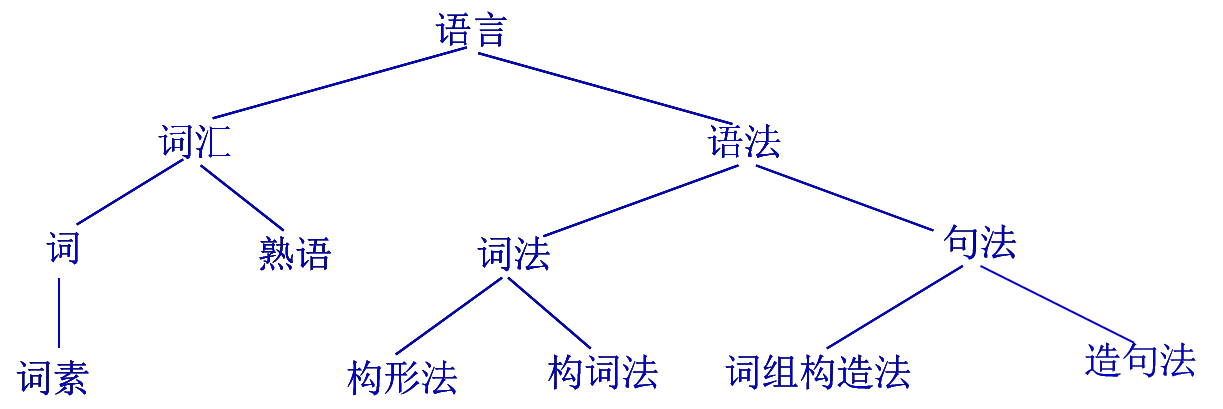
\includegraphics[width=0.76\textwidth]{yuyanc820191130001}
\caption{自然语言的结构}
\label{AI32fig3001}
\end{figure}
%%%%%%%%%%%%%%%%%%%%%%%%%%%%%%%%%%%%%%%%%%

词汇是语言的基本单位. 熟语是指一些词的固定组合, 如汉语中的成语. 词又由词素构成, 词素是构成词的最小有意义的单位. 如“学生”是由“学”和“生”这两个词素构成的.

语法是语言的组织规律. 词法是用词素或熟语构成词的规则, 可分为构形法和构词法. 构形法是指单数复数等. 造句法是用词和词组构造句子的规则.
%%%%%%%%%%%%%%%%%%%%%%%%%%%%%%%%%%%%%%%%%%%%%%
\section{词法分析}
    其主要任务是要找出词汇的各个词素, 从中获得语言学信息, 并确定单词的词义. 以英语为例, 其词法分析的基本算法如下:
\begin{Verbatim}
  repeat
        look for word in dictionary
        if not found
        then modify the word
  until word is found or no further modification possible
\end{Verbatim}
其中, word是一个变量, 其初始值就是当前词.

\begin{example}
  用上述算法分析catches.
\end{example}

解: 其分析过程如下:
\begin{Verbatim}
  catches   词典中查不到
  catche    修改1: 去掉s
  catch     修改2: 去掉e
\end{Verbatim}

可以看出, 在修改2时就查到了catch. 当然, 这只是一个很简单的例子, 完整的词法分析还应该包括复合词的切分等.

%%%%%%%%%%%%%%%%%%%%%%%%%%%%%%%%%%%%%%%%%%%%%%
\section{句法分析}
     句法分析是对句子和短语的结构进行分析, 其最大单位是一个句子. 分析的目的是要找出词、短语等的相互关系, 以及他们在句子中的作用等, 并用一种层次结构加以表达. 这种层次结构可以是句子的成分关系、, 也可以是语法功能关系.
%%%%%%%%%%%%%%%%%%%%%%%%%%%%%%%%%%%%%%%%%%%%%%
\subsection{句法规则的表示方法}
%%%%%%%%%%%%%%%%%%%%%%%%%%%%%%%%%%%%%%%%%%%%%%
\paragraph{句子结构的表示}
一个句子是由各种不同的句子成分组成的. 这些成分可以是单词、词组或从句. 句子成分还可以按其作用分为主语、谓语、宾语、宾语补语、定语、状语、表语等. 这种关系可用一棵树来表示, 如对句子:
\begin{center}
  He  wrote  a  book
\end{center}
可用图\ref{AI32fig2901}所示的树形结构来表示.

一个句子又是由若干个词类构成的, 如名词、动词、代词、形容词等. 若从句子的词类来考虑, 一个句子也可用一棵树来表示, 这种树称为句子的分析树, 如图\ref{AI32fig2901}所示.
%%%%%%%%%%%%%%%%%%%%%%%%%%%%%%%%%%%%%%%%%%
\begin{figure}[H]
\centering
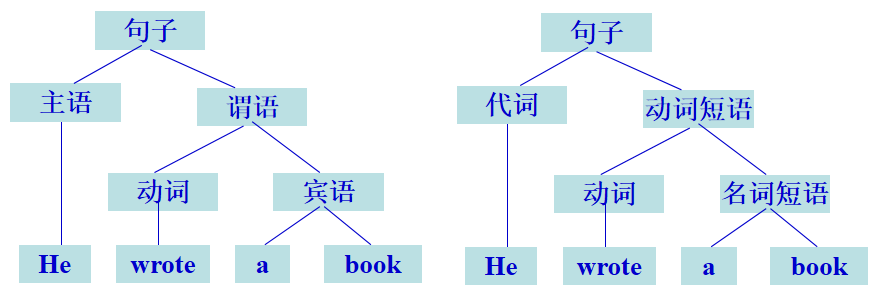
\includegraphics[width=0.76\textwidth]{zhengxiangtuili2019112901.PNG}
\caption{}
\label{AI32fig2901}
\end{figure}
%%%%%%%%%%%%%%%%%%%%%%%%%%%%%%%%%%
\paragraph{上下文无关文法}
上下文无关文法(Context-free  Grammars)是乔姆斯基提出的一种对自然语言语法知识进行形式化描述的方法. 在这种文法中, 语法知识是用重写规则表示的. 作为例子, 下面给出了一个英语的很小的子集(图8.4).

\begin{itemize}
\item 语句 $\rightarrow$\,  句子   终标符
\item 句子 $\rightarrow$\,  名词短语   动词短语
\item 动词短语 $\rightarrow$\,  动词   名词短语
\item 名词短语 $\rightarrow$\,  冠词   名词
\item 名词短语 $\rightarrow$\,  专用名词
\item 冠词 $\rightarrow$\,  the
\item 名词 $\rightarrow$\,  professor
\item 动词 $\rightarrow$\,  wrote
\item 名词 $\rightarrow$\,  book
\item 动词 $\rightarrow$\,  trains
\item 专用名词 $\rightarrow$\,  Jack
\item 终标符 $\rightarrow$\, .
\end{itemize}
这就是一个英语子集的上下文无关文法

在该文法中, “语句”是一个特殊的非终极符, 称为起始符.

句法规则的表示方法

%%%%%%%%%%%%%%%%%%%%%%%%%%%%%%%%%%
\begin{example}
利用上述上下文无关文法, 给出如下语句的分析树.

The  professor  trains  Jack.
\end{example}

解: 如图\ref{AI32fig2902}所示
%%%%%%%%%%%%%%%%%%%%%%%%%%%%%%%%%%%%%%%%%%
\begin{figure}[H]
\centering
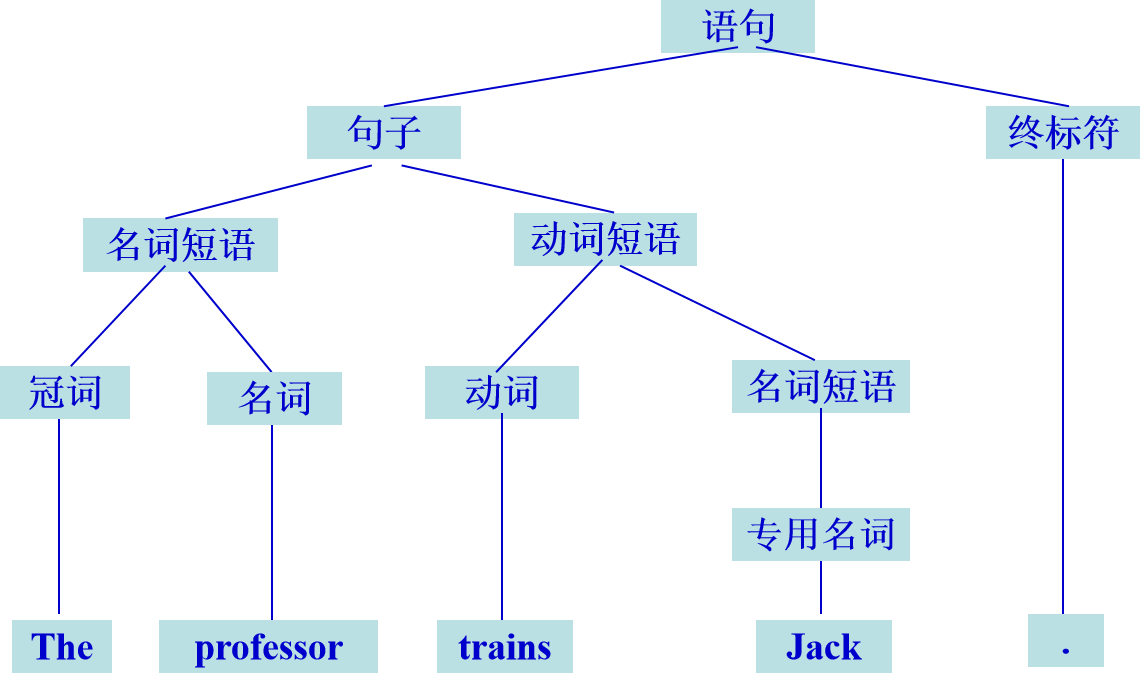
\includegraphics[width=0.76\textwidth]{zhengxiangtuili2019112902.PNG}
\caption{}
\label{AI32fig2902}
\end{figure}
%%%%%%%%%%%%%%%%%%%%%%%%%%%%%%%%%%
%%%%%%%%%%%%%%%%%%%%%%%%%%%%%%%%%%
\paragraph{变换文法}
上下文无关文法反映的仅是一个句子本身的层次结构和生成过程, 而自然语言是上下文有关的. 为此, 乔姆斯基又提出了变换文法(Transformational  Grammar). 该文法认为, 句子的结构有深层和表层两个层次. 例如:
\begin{center}
  She  read  me  a  story  和  She  read  a  story  to  me
\end{center}
的表层结构不一样, 但它们的深层结构则是一样的. 再如, 主动句和被动句也只是表层结构不同, 其深层结构则是相同的.

在变换文法中, 句子深层结构和表层结构之间的变换是通过变换规则实现的, 如图\ref{AI32fig2903}给出了一条把主动句变换为被动句的变换规则.
%%%%%%%%%%%%%%%%%%%%%%%%%%%%%%%%%%%%%%%%%%
\begin{figure}[H]
\centering
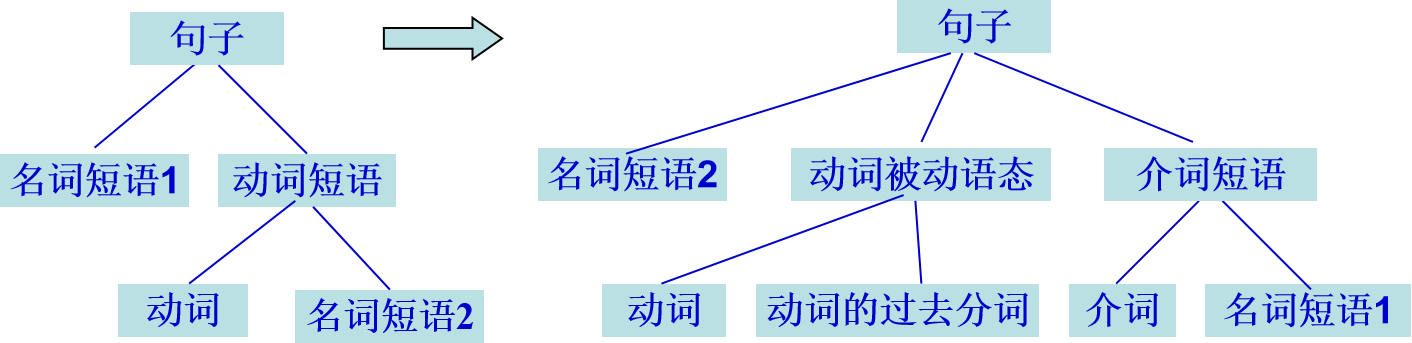
\includegraphics[width=0.76\textwidth]{zhengxiangtuili2019112903.PNG}
\caption{}
\label{AI32fig2903}
\end{figure}
%%%%%%%%%%%%%%%%%%%%%%%%%%%%%%%%%%
%%%%%%%%%%%%%%%%%%%%%%%%%%%%
\begin{example}
  利用变换文法, 将前述主动句变为被动句.
\end{example}

解: 其变换过程是: 先从非终极符“句子”开始产生一个主动句:
\begin{center}
  The  professor  trains  Jack
\end{center}

然后再应用图\ref{AI32fig2904}所示的变换规则把它变为被动句(图\ref{AI32fig2904}) :
\begin{center}
  Jack  is  trained  by  the  professor
\end{center}
%%%%%%%%%%%%%%%%%%%%%%%%%%%%%%%%%%%%%%%%%%
\begin{figure}[H]
\centering
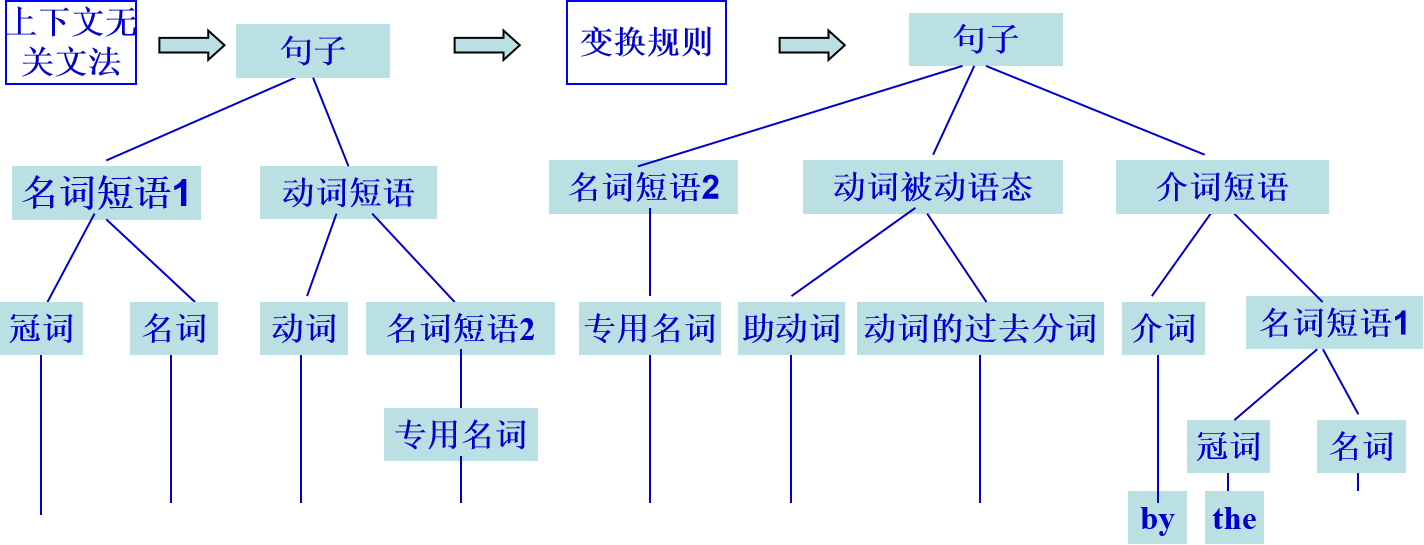
\includegraphics[width=0.76\textwidth]{zhengxiangtuili2019112904.PNG}
\caption{}
\label{AI32fig2904}
\end{figure}
%%%%%%%%%%%%%%%%%%%%%%%%%%%%%%%%%%
%%%%%%%%%%%%%%%%%%%%%%%%%%%%%%%%%%%%%%%%
\paragraph{自顶向下与自底向上分析}
自顶向下分析, 是指从起始符开始应用文法规则, 一层一层地向下产生分析树的各个分支, 直至生成与输入语句相匹配的完整的句子结构为止.

%%%%%%%%%%%%%%%%%%%%%%%%%%%%
\begin{example}
图\ref{AI32fig2909}所示的上下文无关文法, 采用自顶向下分析方法对语句:
\begin{center}
  The  professor  trains  Jack.
\end{center}
\end{example}

进行分析的过程是:
    首先从起始符“语句”开始, 正向运用规则:
\begin{center}
  语句 $\rightarrow$\,  句子   终标符
\end{center}
把分析树的根节点“语句”替换为它的两个子节点“句子”和“终标符”.
    然后再对新生成的节点“句子”使用规则:
\begin{center}
  句子 $\rightarrow$\,  名词短语   动词短语
\end{center}
将其替换为两个子节点“名词短语”与“动词短语”.
    对于“名词短语”, 有两条规则可用, 若按规则的排列顺序, 则选用
\begin{center}
  名词短语 $\rightarrow$\,  冠词    名词
\end{center}
将“名词短语”被替换为“冠词”和“名词”, 生成两个新节点. 对“冠词”使用规则:
\begin{center}
  冠词 $\rightarrow$\,  The
\end{center}
对名词使用规则:
\begin{center}
  名词 $\rightarrow$\,  professor
\end{center}
以此进行$\cdots$, 得到如图8.8所示的自顶向下的分析树.
%%%%%%%%%%%%%%%%%%%%%%%%%%%%%%%%%%%%%%%%
\paragraph{自顶向下与自底向上分析}
自底向上分析, 是以输入语句的单词为基础, 首先按重写规则的箭头指向, 反方向使用那些最具体的重写规则, 把单词归并成较大的结构成分, 如短语等, 然后对这些成分继续逆向使用规则, 直到分析树的根节点为止.

仍以语句
\begin{center}
  The  professor  trains  Jack
\end{center}
为例, 逆向使用图\ref{AI32fig2903}中的那些具体规则后, 可得到图\ref{AI32fig2909}所示的部分分析树.
%%%%%%%%%%%%%%%%%%%%%%%%%%%%%%%%%%%%%%%%%%
\begin{figure}[H]
\centering
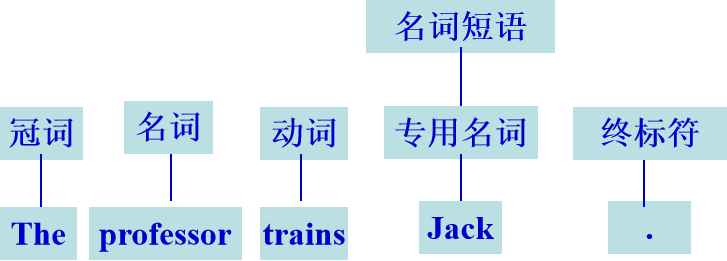
\includegraphics[width=0.76\textwidth]{zhengxiangtuili2019112909.PNG}
\caption{}
\label{AI32fig2909}
\end{figure}
%%%%%%%%%%%%%%%%%%%%%%%%%%%%%%%%%%

继续逆向使用规则, 一步步归并, 直到根节点“语句”为止, 最后即可生成如图\ref{AI32fig2904}所示的完整的分析树.

自顶向下分析方法与自底向上分析方法虽然思路清晰, 但分析效率不高. 为了提高分析效率, 可采用自顶向下与自底向上相结合的分析方法.

%%%%%%%%%%%%%%%%%%%%%%%%%%%%%%%%%%%%%%%%
\section{句义分析}

语义分析就是要识别一句话所表达的实际意义. 即弄清楚“干什么了”, “谁干的”, “这个行为的原因和结果是什么”以及“这个行为发生的时间、地点及其所用的工具或方法”等.

原因是语法分析, 仅是在句法范围内根据词性信息来分析自然语言中句子的文法结构的. 由于它没有考虑句子本身的含义, 也就不能排除像
\begin{center}
  The  paper  received  the  professor
\end{center}
这种在语法结构上正确, 但实际意义上错误的句子.

目前, 用于语义分析的技术比较多, 本节仅简单介绍语义文法和格文法.
%%%%%%%%%%%%%%%%%%%%%%%%%%%%%%%%%%%%%%%%
\subsection{语义文法}
    语义文法是在上下文无关文法的基础上, 将“名词短语”、“动词短语”、“名词”等这些不含有语义信息的纯语法类别, 用所讨论领域的专门信息, 像“山”、“水”、“动物”、等这些具有很强语义约束的语义类别来代替. 利用语义文法进行语义分析, 就可以排除像“论文收到教授”这类无意义的句子.

\begin{example}
下面是一个关于舰船信息的语义文法的例子:
\begin{Verbatim}
        S $\rightarrow $ PRESENT  the  ATTRIBUTE  of  SHIP
        PRESENT $\rightarrow $ what  is  | can  you  tell  me
        ATTRIBUTE $\rightarrow $ length | class
        SHIP $\rightarrow $ the  SHIPNAME | CLASSNAME  class  ship
        SHIPNAME $\rightarrow $ Huanghe | Changjiang
        CLASSNAME $\rightarrow $ carrier | submarine
\end{Verbatim}
在上述重写规则中, 用大写英文字母的单词表示非终极符, 小写英文字母表示终极符, 竖线表示“或”的意思.
\end{example}

利用上述语义文法进行语义分析, 可以从语义上识别以下的输入:
\begin{Verbatim}
  what is the length of the Huanghe?
  Can you tell me the class of the Changjiang?
\end{Verbatim}
%%%%%%%%%%%%%%%%%%%%%%%%%%%%%%%%%%%%%%%%
\subsection{格文法}

%%%%%%%%%%%%%%%%%%%%%%%%%%%%%%%%%%%%%%%%
\paragraph{格和格框架}

    格文法是以句子的中心动词为主导, 并用格来表示其它成分与此中心动词之间的语义关系的一种描述方法.

“格”这个词来源于传统语法, 但它与传统语法中的格有着本质不同. 在传统语法中, 格仅表示一个词或短语再句子中的功能, 如主格、宾格、等, 反映的也只是词尾的变化规则, 故称为表层格. 在格文法中, 格表示的是语义方面的关系, 反映的是句子中所包含的思想、观念等, 故称为深层格.

“格”是一个一般的概念, 相对于中心动词的不同语义关系, 格可以分为许多种. 例如, 在句子
\begin{center}
  John gave the book to Sally
\end{center}
中, 相对于中心动词gave,

\begin{itemize}
\item John是这个行为的发出者, 称为动作格;
\item the book是行为作用的对象, 称为受动格;
\item Sally是行为作用对象所到达的目标, 称为目标格.
\end{itemize}

 一套正确的深层格究竟应包括多少个格, 以及这些格的明确含义是什么, 目前尚无定论.

下面给出一个描述行为的句子, 它所涉及的深层格主要有:
\begin{itemize}
\item Agent(施事),  动作主格, 指行为的施动者;
\item Object(受事), 受动者格, 指行为作用的对象;
\item Co-Agent(共施事), 帮助者格, 指行为施动者的合作者;
\item Instrument(工具), 工具格, 指施事者或共施事者实现行为中所使用的对象;
\item Time(时间),   时间格, 指行为发生的时间;
\item Source(来源), 来源格, 指行为作用对象移出的位置;
\item Goal(目标),   目标格, 指行为作用对象到达的位置;
\item Trajectory(轨迹), 轨迹格, 指从来源到目标所经过的路径.
\end{itemize}

格框架是一种用来描述句子深层格的框架.


在格文法中, 每个句子都联系着一个格框架. 其中, 框架名可以是相应句子的中心动词, 框架的槽可分别对应于相应句子的各个深层格, 每个槽的槽值为该深层格在相应句子中所代表的语义成分.

\begin{example}
前述句子分析结束时所得到的实际格框架为:
\begin{Verbatim}
  [GAVE
            Agent:    John
            Object:    the book
            Source:    John
            Goal:      Sally
        ]
\end{Verbatim}
\end{example}
%%%%%%%%%%%%%%%%%%%%%%%%%%%%%%%%%%%%%%%%
\subsection{长程记忆模型——Compressive Transformer(压缩Transformer)}
长短时记忆(Long Short-Term-Memory, LSTM)的递归神经网络(RNN)是目前最早、应用最为广泛的记忆结构之一. LSTM以数字向量的形式维护一个紧凑的内存, 通过门控读、写和遗忘操作来访问和修改这个内存. 它最初是在一套综合任务上开发的, 包括学习一串bit的逻辑操作. 不过现在它已经被广泛应用在所有的序列数据模型当中了.
LSTM, 以及许多现在所使用的RNNs, 存在一个巨大的缺点, 就是容量问题. 最初设计这些结构的目的是为了, 使每个单元的内存都可以影响其他单元, 并且具有科学系的权重. 但这导致系统的计算效率非常低下, 模型中可学习参数的数量会随内存大小的增加呈平方地增加, 例如内存64KB的LSTM, 会产生8GB的参数( 图\ref{bloglong}).
%%%%%%%%%%%%%%%%%%%%%%%%%%%%%%%%%%%%%%%%%%
\begin{figure}[H]
\centering
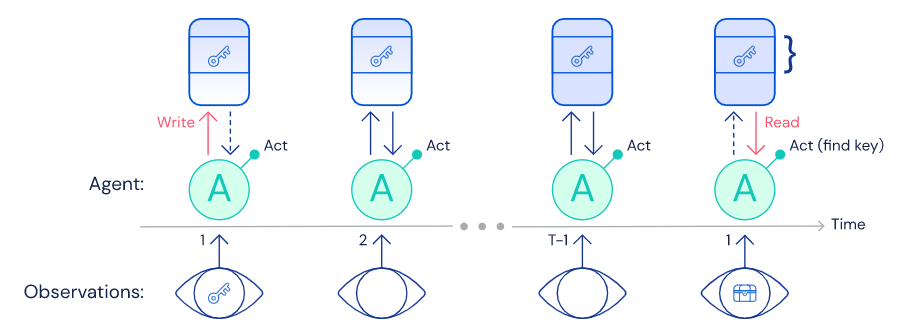
\includegraphics[width=0.76\textwidth]{bloglong.png}
\caption{长期推理对于智能系统的泛化有决定性作用. Here, an agent remembers the existence and location of a key over a long period of time, and recalls this information when a treasure chest is discovered – prompting the agent to return to the remembered location to retrieve the key.}
\label{bloglong}
\end{figure}

DeepMind的研究人员曾提出过一种新的架构, 可微分神经计算机(DNC), 它用更大的内存矩阵来扩充LSTM, 以此来解决这些缺陷.
在我们看东西时, 我们的眼睛会聚焦于视觉场景中的相关物体. 例如, 你可能会花更多的时间注意朋友的面部表情, 而不是注意他们的鞋子.
DNC采用了类似的方法, 使用一个「注意力操作」从这个内存矩阵中读取数据.
在DNC中, 内存模型可以处理过去的特定事件/数据. 这种注意力操作需要固定数量的参数, 而与内存大小无关, 因此可以显著提高模型的内存容量.
随着 DNC的开发, 带有附加注意力机制的递归神经网络在翻译和问题回答领域显示出了巨大的潜力. 这些模型能够使用两种内存结构进行推理, 一种是小型且紧凑的LSTM内存, 一种是大型的外部内存.
最近谷歌Google Brain 的研究人员去除掉 LSTM, 只利用注意力来传输信息, 提出了一种Transformer模型.
Transformer 最初是应用在机器翻译任务上, 性能明显优于递归神经网络.
随后Transformer被广泛应用到NLP的的其他任务当中, 例如问答、文本摘要、情感分析等. 过去一年, 因为Transformer, 这些方面取得了巨大的进步.
但这些模型仍然存在一个缺点, 即它们会把所有的信息都存储起来, 这样在每一个时间步上所消耗的计算成本和存储成本都非常大.
我们的大脑显然不是这样做的, 我们不会像摄像机那样, 把我们一生当中接收到的所有信息存储起来. 而是会根据相关性、惊喜度、危险性、重复次数等因素来选择、过滤、整合所有的输入刺激. 换句话说, 我们会把一生的经历压缩成一组亮点记忆, 帮助我们来理解过去, 以及更好地预测未来.
这就是如何压缩的问题.
之前有一些工作通过稀疏访问机制来尝试压缩注意力中的计算消耗. 但稀疏注意力方法并不能解决存储问题, 而且通常需要定制的稀疏核才能有效地实现.

%%%%%%%%%%%%%%%%%%%%%%%%%%%%%%%%%%%%%%%%
\paragraph{压缩Transformer}

DeepMind提出了Transformer的一个简单变种:  Compressive Transformer模型(压缩 Transformer).
将过去隐藏激活(past hidden activations, 记忆)映射到一个更小的压缩表示集(压缩记忆)中. 在记忆和压缩记忆上, 压缩Transformer会使用相同的注意力机制, 来学习查询它的短期颗粒记忆和长期粗记忆.

压缩Transformer保持对过去激活的细粒度记忆, 然后将其压缩为更粗的压缩记忆. 上面的模型有三层, 一个序列长度$n_s = 3$, 记忆大小$n_m = 6$, 压缩记忆大小$n_{cm} = 6$ \cite{raecompressive2019}. 高亮显示的记忆被压缩, 每层使用压缩函数fc将其压缩到单个压缩记忆中, 而不是在下一个序列中丢弃.
%%%%%%%%%%%%%%%%%%%%%%%%%%%%%%%%%%%%%%%%%%%%%%%%%%
\section{作 业 题}
%%%%%%%%%%%%%%%%%%%%%%%%%%%%%%%%%%%%%%%%%%%%%%%%
\begin{custom}[explorecolor]{探索}
对下列每个语句给出文法分析树:

    (1)  John  wanted  to  go  the  movie  with  Sally.

    (2)  John  wanted  to  go  to  the  movie  with  Robert  Redford.

    (3)  I  heard  the  story  listening  to  the  radio.

    (4)  I  heard  the  kids  listening  to  the  radio.
\end{custom} 